\documentclass[9pt,aspectratio=169,xcolor=table]{beamer}

%~~~~~~~~~~~~~~~~~~~~~~~~~~~~~~~~~~~~~~~~~~~~~~~~~~~~~~~~~~~~~~~~~~~~~~~~~~~~~~
% Use roboto Font (recommended)
\usepackage[sfdefault]{roboto}
\usepackage[utf8]{inputenc}
\usepackage[T1]{fontenc}
%~~~~~~~~~~~~~~~~~~~~~~~~~~~~~~~~~~~~~~~~~~~~~~~~~~~~~~~~~~~~~~~~~~~~~~~~~~~~~~

%~~~~~~~~~~~~~~~~~~~~~~~~~~~~~~~~~~~~~~~~~~~~~~~~~~~~~~~~~~~~~~~~~~~~~~~~~~~~~~
% Define where theme files are located. ('/styles')
\usepackage{styles/fluxmacros}
\usefolder{styles}
% Use Flux theme v0.1 beta
% Available style: asphalt, blue, red, green, gray
\usetheme[style=gray]{flux}
%~~~~~~~~~~~~~~~~~~~~~~~~~~~~~~~~~~~~~~~~~~~~~~~~~~~~~~~~~~~~~~~~~~~~~~~~~~~~~~

%~~~~~~~~~~~~~~~~~~~~~~~~~~~~~~~~~~~~~~~~~~~~~~~~~~~~~~~~~~~~~~~~~~~~~~~~~~~~~~
% Extra packages
\usepackage{booktabs}
\usepackage{colortbl}
\usepackage{ragged2e}
\usepackage{amssymb}
\usepackage{multirow}
\usepackage{tikz}
\usetikzlibrary{arrows.meta, positioning, fit, backgrounds, calc, decorations.pathreplacing}
\setbeamertemplate{itemize items}[square]
\usepackage[scaled=.92]{beramono}
\usepackage{listings}
\usepackage{styles/lstlangarm}
\usepackage{array}
\definecolor{bgcolor}{HTML}{F2E9E9}
% lstlangarm.sty references \color{mauve} for string literals but never defines
% it -- only fires when a listing contains a string. Define it here.
\definecolor{mauve}{rgb}{0.58,0,0.82}
% lstlangarm's C style sets commentstyle=green!20, which is unreadable on the
% pink listing background. Darken it globally.
\lstset{commentstyle=\color{green!45!black}}
% ragged-right fixed-width column -- must be defined in the preamble, never
% inside a frame (\newcolumntype's #1 breaks beamer's frame scanner)
\newcolumntype{R}[1]{>{\RaggedRight\arraybackslash}p{#1}}
%~~~~~~~~~~~~~~~~~~~~~~~~~~~~~~~~~~~~~~~~~~~~~~~~~~~~~~~~~~~~~~~~~~~~~~~~~~~~~~
% Table striping: odd rows white, even rows very light gray.
% Needs \documentclass[...,xcolor=table]{beamer} (beamer loads xcolor itself,
% so the option must go on the class, not \usepackage).
\definecolor{stripe}{gray}{0.94}
% \striped makes body rows alternate white, gray, white, ... starting white.
% \rowcolors counts from the first coloured body row; the header is not counted.
\newcommand{\striped}{\rowcolors{1}{white}{stripe}}
%~~~~~~~~~~~~~~~~~~~~~~~~~~~~~~~~~~~~~~~~~~~~~~~~~~~~~~~~~~~~~~~~~~~~~~~~~~~~~~

%~~~~~~~~~~~~~~~~~~~~~~~~~~~~~~~~~~~~~~~~~~~~~~~~~~~~~~~~~~~~~~~~~~~~~~~~~~~~~~
% TikZ block styles -- matches ch1/ch2
\tikzset{
  blk/.style   = {rectangle, rounded corners=2pt, draw=secondary, fill=secondary!10,
                  align=center, font=\small, minimum height=9mm, inner sep=3pt},
  cpublk/.style= {rectangle, rounded corners=2pt, draw=primary, fill=primary!12,
                  align=center, font=\small\bfseries, minimum height=9mm, inner sep=3pt},
  memblk/.style= {rectangle, rounded corners=2pt, draw=tertiary, fill=tertiary!10,
                  align=center, font=\small, minimum height=9mm, inner sep=3pt},
  cell/.style  = {rectangle, draw=Gray, fill=white, align=center,
                  font=\normalsize\ttfamily, minimum height=7mm, inner sep=2pt},
  lbl/.style   = {font=\scriptsize, text=Gray},
  flow/.style  = {-{Stealth[length=2mm]}, thick, draw=secondary},
  busline/.style={thick, draw=Gray},
}
% NOTE (theme quirks -- all fail SILENTLY, always page through the PDF):
%  - a second \\ inside a nested {...} group in a TikZ node breaks parsing
%  - {\small ...} wrapped around a nested itemize eats the frame title + list
%  - \usebeamercolor on a [plain] frame falls through to an unstyled default
%  - \newcolumntype inside a frame breaks beamer's frame scanner
%  - lstlisting needs \begin{frame}[fragile]
%  - a TikZ picture wider than its column silently overflows into neighbours
%  - 3+ \texttt{} calls in a frame's {title}{subtitle} silently drops the title
%  - a {title}{subtitle} pair on a tikz-only frame body can also drop the
%    title even with 2 or fewer \texttt{} calls -- if a title vanishes,
%    try dropping the subtitle before debugging further
%~~~~~~~~~~~~~~~~~~~~~~~~~~~~~~~~~~~~~~~~~~~~~~~~~~~~~~~~~~~~~~~~~~~~~~~~~~~~~~

%%%%%%%%%%%%%%%%%%%%%%%%%%%%%%%%%%%
%% BEGIN CONDITIONAL COMPILATION %%
%%%%%%%%%%%%%%%%%%%%%%%%%%%%%%%%%%%
\newif\ifwebex
%\webextrue % uncomment to generate section separator
\ifwebex
\AtBeginSection[]{
  \begin{frame}
  \vfill
  \centering
  \begin{beamercolorbox}[sep=8pt,center,shadow=true,rounded=true]{title}
    \usebeamerfont{title}\insertsectionhead\par%
  \end{beamercolorbox}
  \vfill
  \end{frame}
}
\else
\AtBeginSection[]
{
{
    \setbeamercolor{background canvas}{bg=yellow!10}
    \begin{frame}[plain]
        \frametitle{Table of Contents}
        \tableofcontents[currentsection]
    \end{frame}
}
}
\fi
%%%%%%%%%%%%%%%%%%%%%%%%%%%%%%%%%%%
%% END CONDITIONAL COMPILATION   %%
%%%%%%%%%%%%%%%%%%%%%%%%%%%%%%%%%%%

%~~~~~~~~~~~~~~~~~~~~~~~~~~~~~~~~~~~~~~~~~~~~~~~~~~~~~~~~~~~~~~~~~~~~~~~~~~~~~~
% Information
\title{Data Processing}
\subtitle{\emph{Introduction to ARM Cortex-M Microprocessors} --- Chapter 6}
\author{Mun\'{i}m Zabidi}
\institute{\color{primary}Faculty of Electrical Engineering, Universiti Teknologi Malaysia}
\date{\today}
\titlegraphic{assets/logoutmwhite.png}
%~~~~~~~~~~~~~~~~~~~~~~~~~~~~~~~~~~~~~~~~~~~~~~~~~~~~~~~~~~~~~~~~~~~~~~~~~~~~~~

\begin{document}

\titlepage

\begin{frame}{Table of Contents}
    \tableofcontents
\end{frame}

%===============================================================================
\section{Why This Matters}
%===============================================================================

\begin{frame}[fragile]{Why This Chapter Matters}
    \leavevmode
    Last chapter showed how data moves between memory and registers with \texttt{LDR} and \texttt{STR}. This chapter asks the next question: once data is in a register, what can ARM do with it? Arithmetic changes values; logical instructions change individual bits; and a hardware barrel shifter lets ARM fold a shift into almost any instruction, including the ones that calculate an address. After this chapter, when you write \verb+GPIOA->MODER |= (1U << 10)+, you will know exactly which instructions the processor runs, and why each one is needed.
\end{frame}

\begin{frame}{Objectives}
    \leavevmode
    {\small After completing this chapter, you should be able to:}

    \vspace{2mm}
    {\small
    \begin{enumerate}\itemsep2pt
        \item Choose the correct arithmetic instruction, and explain why a 32-bit constant may need more than one instruction.
        \item Write a read-modify-write sequence that changes a bit field without harming adjacent bits.
        \item Predict the result of a shift instruction, and distinguish logical from arithmetic shifts.
        \item Use the flexible second operand, including barrel-shifter forms, to combine a shift with an arithmetic operation.
        \item Use offset addressing, pre-indexed, and post-indexed forms to reach a structure member, and state which registers each mode changes.
        \item Use a scaled register offset to reach an array element, and trace a complete array-processing program.
    \end{enumerate}}
\end{frame}

%===============================================================================
\section{Arithmetic}
%===============================================================================

\begin{frame}{Arithmetic Instructions}
    \begin{center}
    {\small
    \striped
    \begin{tabular}{@{}l l l@{}}
        \toprule
        \textbf{Instruction} & \textbf{Operation} & \textbf{Note} \\
        \midrule
        \texttt{ADD}  & \texttt{Rd = Rn + Operand2}   & \\
        \texttt{SUB}  & \texttt{Rd = Rn $-$ Operand2} & \\
        \texttt{RSB}  & \texttt{Rd = Operand2 $-$ Rn} & \alert{Negation}: \texttt{RSB R0, R1, \#0} \\
        \texttt{MUL}  & \texttt{Rd = Rn $\times$ Rm}  & Single cycle on the M4 \\
        \texttt{SDIV} / \texttt{UDIV} & \texttt{Rd = Rn $\div$ Rm} & 2--12 cycles \\
        \bottomrule
    \end{tabular}}
    \end{center}

    \vspace{3mm}
    \begin{block}{Loading a 32-bit constant}
        The immediate value must fit \emph{inside} the instruction,
        which is itself only 32 bits. So a full constant needs either
        \alert{\texttt{MOVW} then \texttt{MOVT}} (two instructions, no
        memory access), or \alert{\texttt{LDR Rn, =value}} (one
        instruction plus a load from a literal pool).
    \end{block}
\end{frame}

\begin{frame}[fragile]{Arithmetic in C and in Assembly}{Load--process--store, once more}
    \begin{columns}[T]
    \begin{column}{.46\textwidth}
        \textbf{In C}

        \vspace{1mm}
        \begin{lstlisting}[style=myc]
total = a + b - c;
        \end{lstlisting}
    \end{column}
    \begin{column}{.5\textwidth}
        \textbf{In assembly}

        \vspace{1mm}
        \begin{lstlisting}[style=armasm]
	LDR  R0, =a
	LDR  R0, [R0]   ; R0 = a
	LDR  R1, =b
	LDR  R1, [R1]   ; R1 = b
	LDR  R2, =c
	LDR  R2, [R2]   ; R2 = c
	ADD  R3, R0, R1 ; R3 = a + b
	SUB  R3, R3, R2 ; R3 = (a+b) - c
	LDR  R4, =total
	STR  R3, [R4]
        \end{lstlisting}
    \end{column}
    \end{columns}

    \vspace{3mm}
    \begin{block}{One C statement, one register-only computation}
        Every operand is \alert{loaded} into a register before either
        \texttt{ADD} or \texttt{SUB} can touch it. Neither instruction
        ever reads or writes memory directly --- the result is
        \alert{stored} only once, at the very end.
    \end{block}

    \vspace{1mm}
    {\small The compiler is free to reorder or reuse registers, but the
    shape never changes: \alert{load every operand, compute in
    registers, store the result.}}
\end{frame}

%===============================================================================
\section{Logic and Bit Manipulation}
%===============================================================================

\begin{frame}{Logical Instructions}
    \begin{center}
    {\small
    \striped
    \begin{tabular}{@{}l l l@{}}
        \toprule
        \textbf{Instruction} & \textbf{Operation} & \textbf{What it is for} \\
        \midrule
        \texttt{AND} & \texttt{Rd = Rn \& Op2}                & \textbf{Masking} --- keep only bits you care about \\
        \texttt{ORR} & \texttt{Rd = Rn | Op2}                 & \textbf{Setting} bits to 1 \\
        \texttt{EOR} & \texttt{Rd = Rn \^{} Op2}              & \textbf{Toggling} bits \\
        \texttt{BIC} & \texttt{Rd = Rn \& \textasciitilde Op2}& \textbf{Clearing} bits to 0 \\
        \bottomrule
    \end{tabular}}
    \end{center}

    \vspace{3mm}
    \begin{block}{\texttt{BIC} is the one without a matching C operator}
        In C you clear bits with \texttt{x \&= \textasciitilde mask}.
        ARM gives this its own instruction. So the compiler emits
        \emph{one} \texttt{BIC}, where you might expect \texttt{MVN}
        followed by \texttt{AND}.
    \end{block}
\end{frame}

\begin{frame}[fragile]{The Four Operations on the Same Bits}
	R0 contains 12$_{10}$, R1 contains 10$_{10}$.
    \begin{center}
    \begin{tikzpicture}[x=10mm, y=6mm]
    \def\bw{1}

    % Bit numbering above the top row
    \foreach \n [count=\i from 0] in {3,2,1,0}{
        \node[lbl, font=\scriptsize] at (\i*\bw+\bw/2,0.65) {\n};
    }

    % Row: R0
    \node[lbl, anchor=east] at (-0.3,0) {\texttt{R0}};
    \foreach \i/\b in {0/1,1/1,2/0,3/0}{
        \draw[draw=secondary, fill=secondary!10, thick] (\i*\bw,-0.35) rectangle (\i*\bw+\bw,0.35);
        \node[font=\scriptsize\ttfamily] at (\i*\bw+\bw/2,0) {\b};
    }
    \node[lbl, anchor=west] at (4.2*\bw,0) {\texttt{R0 = 1100}};

    % Row: R1
    \node[lbl, anchor=east] at (-0.3,-1.1) {\texttt{R1}};
    \foreach \i/\b in {0/1,1/0,2/1,3/0}{
        \draw[draw=Gray, fill=Gray!8, thick] (\i*\bw,-1.45) rectangle (\i*\bw+\bw,-0.75);
        \node[font=\scriptsize\ttfamily] at (\i*\bw+\bw/2,-1.1) {\b};
    }
    \node[lbl, anchor=west] at (4.2*\bw,-1.1) {\texttt{R1 = 1010}};

    % Row: AND
    \node[lbl, anchor=east] at (-0.3,-2.4) {\texttt{AND}};
    \foreach \i/\b in {0/1,1/0,2/0,3/0}{
        \draw[draw=primary, fill=primary!15, thick] (\i*\bw,-2.75) rectangle (\i*\bw+\bw,-2.05);
        \node[font=\scriptsize\ttfamily\bfseries] at (\i*\bw+\bw/2,-2.4) {\b};
    }
    \node[lbl, anchor=west] at (4.2*\bw,-2.4) {\texttt{R2,R0,R1} --- keep where \alert{both} are 1};

    % Row: ORR
    \node[lbl, anchor=east] at (-0.3,-3.5) {\texttt{ORR}};
    \foreach \i/\b in {0/1,1/1,2/1,3/0}{
        \draw[draw=primary, fill=primary!15, thick] (\i*\bw,-3.85) rectangle (\i*\bw+\bw,-3.15);
        \node[font=\scriptsize\ttfamily\bfseries] at (\i*\bw+\bw/2,-3.5) {\b};
    }
    \node[lbl, anchor=west] at (4.2*\bw,-3.5) {\texttt{R2,R0,R1} --- set where \alert{either} is 1};

    % Row: EOR
    \node[lbl, anchor=east] at (-0.3,-4.6) {\texttt{EOR}};
    \foreach \i/\b in {0/0,1/1,2/1,3/0}{
        \draw[draw=primary, fill=primary!15, thick] (\i*\bw,-4.95) rectangle (\i*\bw+\bw,-4.25);
        \node[font=\scriptsize\ttfamily\bfseries] at (\i*\bw+\bw/2,-4.6) {\b};
    }
    \node[lbl, anchor=west] at (4.2*\bw,-4.6) {\texttt{R2,R0,R1} --- set where they \alert{differ}};

    % Row: BIC
    \node[lbl, anchor=east] at (-0.3,-5.7) {\texttt{BIC}};
    \foreach \i/\b in {0/0,1/1,2/0,3/0}{
        \draw[draw=primary, fill=primary!15, thick] (\i*\bw,-6.05) rectangle (\i*\bw+\bw,-5.35);
        \node[font=\scriptsize\ttfamily\bfseries] at (\i*\bw+\bw/2,-5.7) {\b};
    }
    \node[lbl, anchor=west] at (4.2*\bw,-5.7) {\texttt{R2,R0,R1} --- clear where R1 is 1};
    \end{tikzpicture}
    \end{center}
\end{frame}

\begin{frame}[fragile]{Read--Modify--Write}{The sequence behind every peripheral write}
    \begin{columns}[T]
    \begin{column}{.46\textwidth}
        \textbf{In C}

        \vspace{1mm}
        \begin{lstlisting}[style=myc]
GPIOA->MODER &=
        ~(3U << 10);

GPIOA->MODER |=
        (1U << 10);
        \end{lstlisting}
    \end{column}
    \begin{column}{.5\textwidth}
        \textbf{In assembly}

        \vspace{1mm}
        \begin{lstlisting}[style=armasm]
	LDR  R3, =0x40020000
	LDR  R0, [R3]
	BIC  R0, R0, #0xC00   ; clear bits 11:10
	ORR  R0, R0, #0x400   ; set bit 10
	STR  R0, [R3]
        \end{lstlisting}
    \end{column}
    \end{columns}

    \vspace{3mm}
    \begin{block}{Why you must keep the neighbouring bits}
        This register holds settings for \alert{sixteen pins}. Writing
        the whole register would reconfigure every one of them.
        \alert{Load it, change only your bits, then store it back.}
    \end{block}

    \vspace{1mm}
    \texttt{3U \texttt{<}< 10 = 0xC00}; \quad {\texttt{1U \texttt{<}< 10 = 0x400}. This
    exact sequence sets up \texttt{PA5} as an output.}
\end{frame}

\begin{frame}[fragile]{Following the Bits Through Clear-Then-Set}
    \begin{center}
    \begin{tikzpicture}[x=5.6mm, y=8mm]
    \def\bw{0.9}
    \foreach \row/\ylev/\label/\bits/\note in {%
        0/3/{original}/{0,0,1,1,1,1,1,1,1,1,1,1,1,1,1,1}/{bits 11:10 = \texttt{11}},
        1/2/{\texttt{BIC} mask}/{0,0,0,0,1,1,0,0,0,0,0,0,0,0,0,0}/{1s mark the field},
        2/1/{after \texttt{BIC}}/{0,0,1,1,0,0,1,1,1,1,1,1,1,1,1,1}/{field is now \texttt{00}},
        3/0/{after \texttt{ORR}}/{0,0,1,1,0,1,1,1,1,1,1,1,1,1,1,1}/{field is now \texttt{01}}}{
      \node[lbl, anchor=east, font=\scriptsize] at (-0.35,\ylev+0.3) {\label};
      \foreach \b [count=\i from 0] in \bits {
          \pgfmathsetmacro{\istarget}{(\i==4 || \i==5) ? 1 : 0}
          \ifnum\istarget=1
            \draw[draw=primary, fill=primary!12, thick] (\i*\bw,\ylev) rectangle (\i*\bw+\bw,\ylev+0.6);
          \else
            \draw[draw=secondary, fill=secondary!10, thick] (\i*\bw,\ylev) rectangle (\i*\bw+\bw,\ylev+0.6);
          \fi
          \node[font=\tiny\ttfamily] at (\i*\bw+\bw/2,\ylev+0.3) {\b};
      }
      \node[lbl, anchor=west, font=\scriptsize] at (16*\bw+0.35,\ylev+0.3) {\note};
    }
    % Bit numbering above the top row
    \foreach \n [count=\i from 0] in {15,14,13,12,11,10,9,8,7,6,5,4,3,2,1,0}{
        \node[lbl, font=\scriptsize] at (\i*\bw+\bw/2,3.85) {\n};
    }
    \draw[decorate, decoration={brace, mirror, amplitude=3pt}, draw=primary]
        (4*\bw,-0.15) -- (6*\bw,-0.15);
    \node[lbl, anchor=north, text=primary, font=\scriptsize] at (5*\bw,-0.35)
        {only these two bits ever change};
    \end{tikzpicture}
    \end{center}

    \vspace{2mm}
    {\small \texttt{ORR} alone cannot turn \texttt{11} into \texttt{01} --- OR can only
    turn bits \alert{on}. \texttt{BIC} must clear the field first.}
\end{frame}

\begin{frame}{Assembly Step by C Step}
    \begin{center}
    {\small
    \striped
    \begin{tabular}{@{}l l l@{}}
        \toprule
        \textbf{Step} & \textbf{Assembly} & \textbf{Equivalent C} \\
        \midrule
        Load the register & \texttt{LDR R1, [R0]} & implicit in \texttt{GPIOA->MODER} \\
        Clear the field & \texttt{BIC R1, R1, R2} & \texttt{\&= \textasciitilde(3U << 10)} \\
        Set the new value & \texttt{ORR R1, R1, \#0x400} & \texttt{|= (1U << 10)} \\
        Store the register & \texttt{STR R1, [R0]} & implicit in the \texttt{->} assignment \\
        \bottomrule
    \end{tabular}}
    \end{center}

    \vspace{3mm}
    \begin{block}{Two rows are ``implicit''}
        C never issues a separate load or store on its own --- the compiler
        emits \texttt{LDR}/\texttt{STR} automatically around every
        \texttt{->MODER} reference. Only the middle two rows have a direct
        C spelling.
    \end{block}
\end{frame}

%===============================================================================
\section{Shift Basics}
%===============================================================================

\begin{frame}{The Four Shifts}
	\leavevmode
	{\small Shift operations move all bits in a register left or right by a specified number of positions, useful for fast arithmetic and bit manipulation.}

	\vspace{2mm}
	\begin{block}{Connection to Digital Electronics}
		{\small You have already encountered these concepts in Digital Electronics as hardware shift registers (SISO, SIPO, PISO, PIPO) and ring counters.}
	\end{block}

	\vspace{2mm}
	\begin{center}
		{\small
			\striped
			\begin{tabular}{@{}l l R{.6\textwidth}@{}}
				\toprule
				\textbf{Instruction} & \textbf{Meaning} & \textbf{Effect} \\
				\midrule
				\texttt{LSL \#n} & Logical shift left   & Multiplies by $2^n$; zeros fill in from the right \\
				\texttt{LSR \#n} & Logical shift right  & Divides an \alert{unsigned} value by $2^n$; zeros fill in from the left \\
				\texttt{ASR \#n} & Arithmetic shift right & Divides a \alert{signed} value by $2^n$; the sign bit fills in from the left \\
				\texttt{ROR \#n} & Rotate right        & Bits that fall off the right re-enter on the left \\
				\bottomrule
		\end{tabular}}
	\end{center}

	\vspace{2mm}
	\begin{block}{Only one bit decides LSR versus ASR}
		{\small Both shift right. The difference is what fills the vacated
			bits: \texttt{LSR} always fills with \alert{0}. \texttt{ASR}
			copies the \alert{sign bit}, so a negative number stays
			negative after the shift.}
	\end{block}
\end{frame}

\begin{frame}[fragile]{Shifts as Ordinary Instructions}
    \leavevmode
    \begin{lstlisting}[style=armasm]
	LSL R0, R1, #2    ; R0 = R1 << 2   (R1 times 4)
	LSR R0, R1, #1    ; R0 = R1 >> 1   (R1 divided by 2, unsigned)
	ASR R0, R1, #1    ; R0 = R1 >> 1   (R1 divided by 2, signed)
    \end{lstlisting}

    \vspace{3mm}
    {\small Written this way, a shift is a complete instruction: it
    reads \texttt{R1}, shifts it, and writes the result to \texttt{R0}
    --- exactly like \texttt{ADD} or \texttt{MOV}.}

    \vspace{3mm}
    \begin{block}{The idea worth carrying forward}
        A shift is useful by itself. But ARM can also feed a shifted
        value \alert{directly into another instruction}, without a
        separate shift step first. That is the subject of the next
        section.
    \end{block}
\end{frame}

\definecolor{nibhifill}{HTML}{DCEBFF}
\definecolor{nibhiline}{HTML}{1565C0}
\definecolor{niblofill}{HTML}{FFE0B2}
\definecolor{nibloline}{HTML}{E65100}
\definecolor{nibrestfill}{HTML}{EDEDED}
\definecolor{nibrestline}{HTML}{9E9E9E}

\begin{frame}[fragile]{Swapping Two Nibbles}{Isolate with \texttt{AND}, recombine with \texttt{ORR}}
    \begin{center}
    \begin{tikzpicture}[x=10mm, y=6mm]
        % Bit-range numbering above the top row; each cell is one nibble
        \foreach \hi/\lo [count=\i from 0] in {31/28,27/24,23/20,19/16,15/12,11/8,7/4,3/0}{
            \node[lbl, font=\tiny] at (\i+0.5,0.65) {\hi:\lo};
        }

        % Row 0: original R0, low byte split into two nibbles, rest greyed
        \node[lbl, anchor=east] at (-0.3,0) {\texttt{R0}};
        \foreach \i/\c in {0/nibrest,1/nibrest,2/nibrest,3/nibrest,4/nibrest,5/nibrest,6/nibhi,7/niblo}{
            \draw[draw=\c line, fill=\c fill, thick] (\i,-0.35) rectangle (\i+1,0.35);
        }
        \node[font=\scriptsize\ttfamily] at (6.5,0) {A};
        \node[font=\scriptsize\ttfamily] at (7.5,0) {B};
        \node[lbl, anchor=west] at (8.2,0) {original low byte \texttt{0xAB}};

        % Row 1: after the two ANDs, isolated on separate rows
        \node[lbl, anchor=east] at (-0.3,-1.1) {\texttt{R1}};
        \foreach \i in {0,...,5}{
            \draw[draw=nibrestline, fill=nibrestfill, thick] (\i,-1.45) rectangle (\i+1,-0.75);
        }
        \draw[draw=nibhiline, fill=nibhifill, thick] (6,-1.45) rectangle (7,-0.75);
        \node[font=\scriptsize\ttfamily] at (6.5,-1.1) {A};
        \draw[draw=nibrestline, fill=nibrestfill, thick] (7,-1.45) rectangle (8,-0.75);
        \node[font=\scriptsize\ttfamily] at (7.5,-1.1) {0};
        \node[lbl, anchor=west] at (8.2,-1.1) {\texttt{AND R1,R0,\#0xF0}};

        \node[lbl, anchor=east] at (-0.3,-2.0) {\texttt{R2}};
        \foreach \i in {0,...,5}{
            \draw[draw=nibrestline, fill=nibrestfill, thick] (\i,-2.35) rectangle (\i+1,-1.65);
        }
        \draw[draw=nibrestline, fill=nibrestfill, thick] (6,-2.35) rectangle (7,-1.65);
        \node[font=\scriptsize\ttfamily] at (6.5,-2.0) {0};
        \draw[draw=nibloline, fill=niblofill, thick] (7,-2.35) rectangle (8,-1.65);
        \node[font=\scriptsize\ttfamily] at (7.5,-2.0) {B};
        \node[lbl, anchor=west] at (8.2,-2.0) {\texttt{AND R2,R0,\#0x0F}};

        % Row 2: after the shifts reposition each nibble
        \node[lbl, anchor=east] at (-0.3,-3.1) {\texttt{R1}};
        \foreach \i in {0,...,5}{
            \draw[draw=nibrestline, fill=nibrestfill, thick] (\i,-3.45) rectangle (\i+1,-2.75);
        }
        \draw[draw=nibrestline, fill=nibrestfill, thick] (6,-3.45) rectangle (7,-2.75);
        \node[font=\scriptsize\ttfamily] at (6.5,-3.1) {0};
        \draw[draw=nibhiline, fill=nibhifill, thick] (7,-3.45) rectangle (8,-2.75);
        \node[font=\scriptsize\ttfamily] at (7.5,-3.1) {A};
        \node[lbl, anchor=west] at (8.2,-3.1) {\texttt{LSR R1,R1,\#4} --- A moves down};

        \node[lbl, anchor=east] at (-0.3,-4.0) {\texttt{R2}};
        \foreach \i in {0,...,5}{
            \draw[draw=nibrestline, fill=nibrestfill, thick] (\i,-4.35) rectangle (\i+1,-3.65);
        }
        \draw[draw=nibloline, fill=niblofill, thick] (6,-4.35) rectangle (7,-3.65);
        \node[font=\scriptsize\ttfamily] at (6.5,-4.0) {B};
        \draw[draw=nibrestline, fill=nibrestfill, thick] (7,-4.35) rectangle (8,-3.65);
        \node[font=\scriptsize\ttfamily] at (7.5,-4.0) {0};
        \node[lbl, anchor=west] at (8.2,-4.0) {\texttt{LSL R2,R2,\#4} --- B moves up};

        % Row 3: final ORR result
        \node[lbl, anchor=east] at (-0.3,-5.1) {\texttt{R0}};
        \foreach \i/\c in {0/nibrest,1/nibrest,2/nibrest,3/nibrest,4/nibrest,5/nibrest}{
            \draw[draw=\c line, fill=\c fill, thick] (\i,-5.45) rectangle (\i+1,-4.75);
        }
        \draw[draw=nibloline, fill=niblofill, thick] (6,-5.45) rectangle (7,-4.75);
        \node[font=\scriptsize\ttfamily\bfseries] at (6.5,-5.1) {B};
        \draw[draw=nibhiline, fill=nibhifill, thick] (7,-5.45) rectangle (8,-4.75);
        \node[font=\scriptsize\ttfamily\bfseries] at (7.5,-5.1) {A};
        \node[lbl, anchor=west, text=nibloline] at (8.2,-5.1) {\texttt{ORR R0,R1,R2} --- swapped, \texttt{0xBA}};
    \end{tikzpicture}
    \end{center}
\end{frame}

\begin{frame}[fragile]{Multiplying by a Power of Two}{Strength reduction: replacing multiply with shift}
    \begin{columns}[T]
    \begin{column}{.46\textwidth}
        \textbf{In C}

        \vspace{1mm}
        \begin{lstlisting}[style=myc]
total = 4 * a + b;
        \end{lstlisting}

        \vspace{2mm}
        {\small \texttt{a} and \texttt{b} are already in \texttt{R0} and
        \texttt{R1} --- no \texttt{LDR} needed here.}
    \end{column}
    \begin{column}{.5\textwidth}
        \textbf{In assembly}

        \vspace{1mm}
        \begin{lstlisting}[style=armasm]
	LSL  R2, R0, #2  ; R2 = a << 2
	                 ;    = a * 4
	ADD  R3, R2, R1  ; R3 = (4*a) + b
        \end{lstlisting}
    \end{column}
    \end{columns}

    \vspace{3mm}
    \begin{block}{Why the compiler prefers \texttt{LSL} over \texttt{MUL}}
        Multiplying by \alert{4} is multiplying by $2^2$. A left shift
        by 2 bits produces exactly that result, and on most cores a
        shift is \alert{cheaper} than a general multiply. The compiler
        makes this substitution automatically --- it is called
        \alert{strength reduction}. No \texttt{MUL} instruction appears
        at all.
    \end{block}

    \vspace{1mm}
    {\small This only works for a power-of-two constant. \texttt{4 * a}
    becomes a shift; \texttt{5 * a} still needs a real \texttt{MUL}.}
\end{frame}
%===============================================================================
\section{The Barrel Shifter}
%===============================================================================

\begin{frame}{What is the Barrel Shifter?}
	\leavevmode
	{\small A \textbf{barrel shifter} is a specialized digital circuit that can shift or rotate a data word by \alert{any number of bit positions in a single clock cycle}.}

	\vspace{2mm}
	\begin{block}{Why is it a game-changer in ARM?}
		\begin{itemize}
			\setlength{\itemsep}{2pt}
			\item \textbf{Hardware Efficiency:} Unlike a basic shift register (which shifts 1 bit per cycle), it uses combinational multiplexers to shift $n$ bits instantly.
			\item \textbf{Zero-Cost Operations:} In ARM processors, it is wired directly into the ALU input path.
			\item \textbf{Combined Execution:} Shifts and arithmetic/logic operations happen in the \alert{same instruction cycle} with zero clock penalty.
		\end{itemize}
	\end{block}

	\vspace{2mm}
	\begin{center}
		{\small \texttt{ADD R0, R1, R2, LSL \#2} \quad $\longrightarrow$ \quad Shift \texttt{R2} left by 2, then add to \texttt{R1} in \alert{1 cycle}.}
	\end{center}
\end{frame}

\begin{frame}[fragile]{The Flexible Second Operand}
	\leavevmode
	{\ttfamily\large Opcode\{S\}\{cond\} \quad Rd, \quad Rn, \quad Operand2}

	\vspace{2mm}
	\begin{center}
		{\small
			\striped
			\begin{tabular}{@{}l l R{.44\textwidth}@{}}
				\toprule
				\textbf{Form} & \textbf{Written} & \textbf{Meaning} \\
				\midrule
				Constant & \texttt{\#constant} & An immediate encoded in the instruction \\
				Register & \texttt{Rm} & A register holding the second operand \\
				Register with shift & \texttt{Rm, LSL \#n} & \texttt{Rm} shifted before use \\
				\bottomrule
		\end{tabular}}
	\end{center}

	\vspace{2mm}
	\begin{lstlisting}[style=armasm]
		ADD R0, R1, R2, LSR #3    ; R0 = R1 + (R2 >> 3)
		ORR R0, R1, R2, LSL #2    ; R0 = R1 | (R2 << 2)
	\end{lstlisting}

	\vspace{2mm}
	\begin{block}{Folded into the instruction, not a separate step}
		{\small The \alert{barrel shifter} sits in the datapath \emph{before}
			the ALU, so the shift and the operation happen together: no
			separate shift instruction is needed. \texttt{Rm} itself stays
			\alert{unchanged} --- only the value entering the ALU is
			shifted.}
	\end{block}
\end{frame}

\definecolor{regfill}{HTML}{FFF1B6}
\definecolor{regline}{HTML}{AB9042}
\definecolor{shiftfill}{HTML}{C3E9FF}
\definecolor{shiftline}{HTML}{3F7691}
\definecolor{alufill}{HTML}{D8FFD2}
\definecolor{aluline}{HTML}{4F7D49}
\definecolor{psrfill}{HTML}{ECDCE8}
\definecolor{psrline}{HTML}{CFABCF}
\definecolor{busflag}{HTML}{A84A4A}

\tikzset{
	lbl/.style={text=black},
	flow/.style={-{Stealth[length=2mm]}, thick},
}

\begin{frame}[plain]{Where the Barrel Shifter Sits}
	\begin{center}
		\resizebox{0.68\textwidth}{!}{%
			\begin{tikzpicture}[xscale=0.11,yscale=-0.11]

				% --- Register Bank ---
				\draw[thick, draw=regline, fill=regfill, rounded corners=3pt]
				(0.2,2.8) rectangle (26.7,26.7);
				\node[lbl, font=\sffamily\bfseries, align=center] at (13.4,12.9) {Register\\Bank};

				% --- Barrel Shifter (parallelogram) ---
				\draw[thick, draw=shiftline, fill=shiftfill]
				(58.4,0.2) -- (90.2,0.2) -- (82.2,16.1) -- (50.5,16.1) -- cycle;
				\node[lbl, font=\sffamily\bfseries, align=center] at (70.3,8.1) {Barrel\\Shifter};

				% --- ALU (chevron-notched hexagon) ---
				\draw[thick, draw=aluline, fill=alufill]
				(42.5,31.9) -- (59.7,31.9) -- (61.1,34.6) -- (62.4,31.9) --
				(79.6,31.9) -- (71.6,53.1) -- (50.5,53.1) -- cycle;
				\node[lbl, font=\sffamily\bfseries] at (61.1,44.0) {ALU};
				\node[lbl, font=\sffamily\small] at (51.4,34.9) {Op1};
				\node[lbl, font=\sffamily\small] at (70.8,34.9) {Op2};
				\node[lbl, font=\sffamily\small] at (61.1,49.4) {Result};

				% --- xPSR (flags register) ---
				\draw[thick, draw=psrline, fill=psrfill, rounded corners=2pt]
				(95.4,37.2) rectangle (116.6,47.8);
				\node[lbl, font=\sffamily\bfseries] at (106.0,42.9) {xPSR};

				% --- Bus: Rm  (Register Bank -> Barrel Shifter -> ALU Op2) ---
				\draw[flow, draw=shiftline] (26.7,7.1) -- (55.0,7.1);
				\node[lbl, font=\sffamily\small, anchor=south] at (36,6.2) {Rm};
				\draw[flow, draw=shiftline] (69.5,16.1) -- (69.5,31.9);

				% --- Bus: Rn / Rd  (Register Bank <-> ALU) ---
				\draw[flow, draw=aluline] (26.6,20.9) -- (50.4,20.9) -- (50.4,31.9);
				\node[lbl, font=\sffamily\small, anchor=south] at (35,19.9) {Rn};
				\draw[flow, draw=aluline] (60.8,53.1) -- (60.8,58.4) -- (14.0,58.4) -- (14.0,26.7);
				\node[lbl, font=\sffamily\small, anchor=north] at (37,58.9) {Rd};

				% --- Bus: flags / carry-in  (ALU <-> xPSR, xPSR -> Shifter) ---
				\draw[flow, draw=busflag] (76.0,{42.5-1.0}) -- (95.4,{42.5-1.0});
				\draw[flow, draw=busflag] (95.4,{42.5+1.0}) -- (76.0,{42.5+1.0});
				\node[lbl, font=\sffamily\scriptsize, text=busflag] at (85.5,{42.5-3.2}) {flags};
				\node[lbl, font=\sffamily\scriptsize, text=busflag] at (85.5,{42.5+3.4}) {carry-in};
				\draw[flow, draw=busflag] (106.0,37.2) -- (106.0,5.5) -- (89.6,5.5);
				\node[lbl, font=\sffamily\scriptsize, text=busflag, anchor=south] at (97,4.6) {C (RRX)};

			\end{tikzpicture}%
		}
	\end{center}
	\vspace{1mm}
	{\small\centering \texttt{Rm} feeds the barrel shifter. Its output
		enters the ALU as \texttt{Op2}. \texttt{Rn} feeds \texttt{Op1}
		directly. The result is written back to \texttt{Rd}, and the flags
		update in \texttt{xPSR}. The carry bit of xPSR is sent to ALU and barrel shifter.\par}
\end{frame}

%===============================================================================
\section{Addressing Modes}
%===============================================================================

\begin{frame}{The Four Addressing Modes}
    \leavevmode
    Assume \texttt{R1} $=$ \texttt{0x2000} before each instruction.

    \vspace{3mm}
    \begin{center}
    {\small
    \striped
    \begin{tabular}{@{}l l l l@{}}
        \toprule
        \textbf{Instruction} & \textbf{Mode} & \textbf{Reads from} & \textbf{R1 afterwards} \\
        \midrule
        \texttt{LDR R0, [R1]}       & register     & \texttt{0x2000} & \texttt{0x2000} \\
        \texttt{LDR R0, [R1, \#8]}  & offset       & \texttt{0x2008} & \texttt{0x2000} \\
        \texttt{LDR R0, [R1, \#8]!} & pre-indexed  & \texttt{0x2008} & \alert{\texttt{0x2008}} \\
        \texttt{LDR R0, [R1], \#8}  & post-indexed & {\texttt{0x2000}} & \alert{\texttt{0x2008}} \\
        \bottomrule
    \end{tabular}}
    \end{center}

    \vspace{3mm}
  \begin{block}{The Writeback Indicator (\texttt{!})}
	\begin{itemize}
		\item The exclamation point \texttt{!} explicitly commands auto-update (writeback) for pre-indexed access.
		\item Post-indexed access \textbf{implicitly updates} the base register without requiring a \texttt{!} symbol.
	\end{itemize}
\end{block}
\end{frame}


\begin{frame}[fragile]{Syntax Cheat Sheet}
    \begin{columns}[b]
    \begin{column}{0.48\textwidth}
        \textbf{1. Simple offset}
        \begin{lstlisting}[style=armasm]
	LDR R0, [R1, #8]
	; address = R1 + 8
	; R1 unchanged
        \end{lstlisting}

        \vspace{5mm}
        \textbf{2. Pre-indexed}: Calculate first, then access.
        \begin{lstlisting}[style=armasm]
	LDR R0, [R1, #8]!
	; address = R1 + 8
	; R1 = R1 + 8
        \end{lstlisting}
        \vspace{5mm}
                \textbf{3. Post-indexed}: Access first, then calculate.
        \begin{lstlisting}[style=armasm]
	LDR R0, [R1], #8
	; address = R1
    ; R1 = R1 + 8 (after)
        \end{lstlisting}

    \end{column}
    \begin{column}{0.48\textwidth}

        \begin{block}{Read the brackets, not the mnemonic}
            \begin{itemize}\itemsep1pt
                \item Offset \alert{inside} the brackets $\rightarrow$
                      pre-indexed.
                \item Offset \alert{outside} the brackets $\rightarrow$
                      post-indexed.
                \item Trailing \texttt{!} $\rightarrow$ writeback.
            \end{itemize}
        \end{block}
    \end{column}
    \end{columns}
\end{frame}

\begin{frame}[plain]{Visualizing Offset Access}{\texttt{LDR R0, [R1, \#8]}}
	\begin{center}
		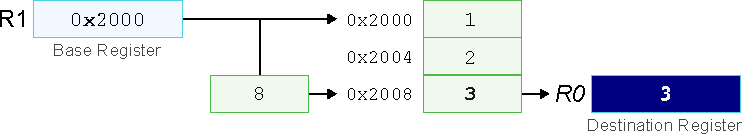
\includegraphics[width=.82\textwidth]{assets/offset.pdf}
	\end{center}
	\vspace{1mm}
	{\small\centering \texttt{R0} is loaded with the address pointed by \texttt{R1 + 8}
		--- \texttt{0x2008}. \texttt{R1} is not updated.\par}
\end{frame}

\begin{frame}[plain]{Visualizing Pre-Indexed Access}{\texttt{STR R0, [R1, \#16]!}}
    \begin{center}
    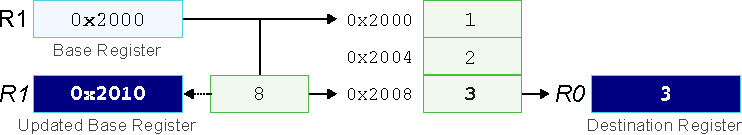
\includegraphics[width=.82\textwidth]{assets/preindexed.pdf}
    \end{center}
    \vspace{1mm}
    {\small\centering The address is computed \emph{first}:
    \texttt{0x2000 + 16 = 0x2010}. This is both where
    \texttt{R0} is loaded from, and where \texttt{R1} ends up. One
    calculation, used twice.\par}
\end{frame}

\begin{frame}[plain]{Visualizing Post-Indexed Access}{\texttt{STR R0, [R1], \#16}}
    \begin{center}
    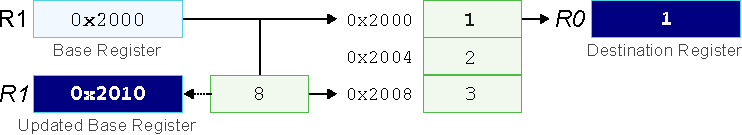
\includegraphics[width=.82\textwidth]{assets/postindexed.pdf}
    \end{center}
    \vspace{1mm}
    {\small\centering \texttt{R0} is loaded from address \texttt{R1}
    already held --- \texttt{0x2000} --- \emph{before} anything
    changes. \texttt{R1} is updated \emph{afterward}, to
    \texttt{0x2010}, ready for the next access.\par}
\end{frame}

\begin{frame}{These Modes Are Not Just for Arrays}
	\leavevmode
	{\small Offset, pre-indexed, and post-indexed addressing are useful
		for any pointer, not only array indices:}

	\vspace{2mm}
	\begin{itemize}\itemsep2pt
		\item A \alert{structure field} at a fixed offset from a base
		pointer --- \texttt{[R1, \#4]}

		\item A \alert{buffer} walked one element at a time, letting
		the pointer advance itself --- \texttt{[R1], \#4}

		\item A \alert{local variable in a stack frame} at a fixed
		offset from the frame pointer --- \texttt{[R7, \#8]}
	\end{itemize}

	\vspace{3mm}
	{\small Every one of these uses a constant offset. No second
		register or shift is needed. The next section adds a register
		offset---and then a scaled register offset---when the offset itself
		is \alert{data}, such as a run-time index.}
\end{frame}

%===============================================================================
\section{Dynamic Indexed Modes}
%===============================================================================
\begin{frame}{Dynamic Indexed Access}
	\begin{center}
		{\small
			\striped
			\begin{tabular}{@{}l l l@{}}
				\toprule
				\textbf{Form} & \textbf{Written} & \textbf{Typical C equivalent} \\
				\midrule
				Immediate offset
				& \texttt{[R1, \#4]}
				& \texttt{*(p + 1)} \\[1mm]
				Register offset
				& \texttt{[R1, R2]}
				& \texttt{*((char *)p + offset)} \\[1mm]
				Scaled register offset
				& \texttt{[R1, R2, LSL \#2]}
				& \texttt{p[i]} \\
				\bottomrule
		\end{tabular}}
	\end{center}

	\vspace{4mm}

	\begin{block}{The key idea}
		{\small
			A register offset supplies a displacement at run time.
			A \alert{scaled} register offset also multiplies that
			displacement by a power of two, which makes it ideal for
			array indexing.}
	\end{block}

	\vspace{2mm}

	{\small
		For a 32-bit element:
		\[
		\text{address} = \text{base} + (\text{index} \times 4)
		\]
	}
\end{frame}


\begin{frame}[fragile]{Scaled Register Offset}
	\begin{columns}[T]
		\begin{column}{.48\textwidth}
			\begin{lstlisting}[style=armasm]
	LDR R0, [R1, R2, LSL #2]
			\end{lstlisting}

			\vspace{3mm}
			{\small
				\begin{itemize}\itemsep1pt
					\item \texttt{R1} --- base address of the array
					\item \texttt{R2} --- the index
					\item \texttt{LSL \#2} --- scale by 4, the element size
			\end{itemize}}

			\vspace{2mm}
			{\small An immediate offset is fixed when you write the
				program; a register offset can change \alert{while the
					program runs}, which is exactly what a loop counter needs.}
		\end{column}
		\begin{column}{.48\textwidth}
			\begin{block}{Indexing without a multiply}
				The barrel shifter feeds directly into address generation,
				so scaling the index, adding the base, and loading the value
				all happen in \alert{one instruction}. No separate shift or
				\texttt{MUL} is needed.

				\vspace{2mm}
				This is Chapter 3's formula, \texttt{base + (index * element size)},
				computed by hardware. It is why that multiplication never
				appears explicitly in compiler output.
			\end{block}
		\end{column}
	\end{columns}

	\vspace{3mm}
	\begin{center}
		{\small
			\begin{tabular}{@{}l l@{}}
				\toprule
				\textbf{Shift} & \textbf{Scales by, matching} \\
				\midrule
				\texttt{LSL \#1} & 2 --- a 16-bit halfword (\texttt{int16\_t}) \\
				\texttt{LSL \#2} & 4 --- a 32-bit word (\texttt{int32\_t}, any pointer) \\
				\bottomrule
		\end{tabular}}
	\end{center}
\end{frame}

\begin{frame}[fragile]{Array Indexing Becomes a Scaled Offset}
	\begin{columns}[T]
		\begin{column}{.46\textwidth}
			\textbf{C}

			\begin{lstlisting}[style=myc]
	int x = array[i];
			\end{lstlisting}

			\vspace{2mm}
			{\small
				For a 32-bit \texttt{int}, the compiler computes the
				address as $\texttt{array} + i \times 4$.
			}

			\vspace{5mm}
		{\small
	\begin{tabular}{@{}l l@{}}
		\toprule
		\textbf{C type} & \textbf{Typical scaling} \\
		\midrule
		\texttt{int16\_t *} & \texttt{LSL \#1} \quad (2 bytes) \\
		\texttt{int32\_t *} & \texttt{LSL \#2} \quad (4 bytes) \\
		\texttt{uint32\_t *} & \texttt{LSL \#2} \quad (4 bytes) \\
		\bottomrule
\end{tabular}}
		\end{column}

		\begin{column}{.50\textwidth}
			\textbf{Typical ARM}

			\begin{lstlisting}[style=armasm]
	; R1 = array
	; R2 = i
	LDR R0, [R1, R2, LSL #2]
			\end{lstlisting}
			\vspace{2mm}
			\begin{block}{Address calculation}
				\[
				R1 + (R2 \times 4)
				\]
				The shift scales the index before it is added to the
				base address.
			\end{block}
		\end{column}
	\end{columns}

	\vspace{3mm}

	\begin{center}
	\end{center}
	\vspace{2mm}

This is why array access on ARM is so cheap.
{\small If someone says ``the barrel shifter is just a historical    curiosity,'' they have not looked at what the compiler produces for    an array loop.}



\end{frame}

\begin{frame}[fragile]{Array Indexing vs Pointer Arithmetic}
	\begin{columns}[T]
		\begin{column}{.47\textwidth}
			\textbf{Same address, different notation}
			\begin{lstlisting}[style=myc]
	int x = array[i];
	int x = *(array + i);

	int *p = array;
	int x = p[i];   // same as *(p + i)
			\end{lstlisting}

			\vspace{2mm}
			{\small
				In every case, \texttt{i} is an \emph{element index}.
				Pointer arithmetic automatically accounts for the size
				of the pointed-to type.
			}
		\end{column}

		\begin{column}{.49\textwidth}
			\textbf{What changes at the machine level?}

			\vspace{1mm}
			{\small
				The compiler turns the element index into a byte
				displacement:
				\[
				i \times \texttt{sizeof(int)}
				\]
			}

			\vspace{2mm}

			\begin{block}{A useful distinction}
				\small
				\texttt{p + i} advances by \texttt{i} \emph{elements}.

				\vspace{1mm}

				\texttt{(char *)p + i} advances by \texttt{i} \emph{bytes}.
			\end{block}
		\end{column}
	\end{columns}

\end{frame}





\begin{frame}[fragile]{Worked Example: Array Processing}
	\begin{columns}[T]
		\begin{column}{.48\textwidth}
			\textbf{C code}
			\begin{lstlisting}[style=myc]
	int array[10];
	int sum = 0;
	int i;

	for (i = 0; i < 10; i++) {
		sum += array[i];
	}
			\end{lstlisting}
		\end{column}
		\begin{column}{.48\textwidth}
			\textbf{ARM assembly}
			\begin{lstlisting}[style=armasm]
	LDR  R1, =array     ; base address
	MOV  R0, #0         ; sum = 0
	MOV  R2, #0         ; i = 0
loop
	LDR  R3, [R1, R2, LSL #2]
	ADD  R0, R0, R3     ; sum += a[i]
	ADD  R2, R2, #1     ; i++
	CMP  R2, #10
	BLT  loop
			\end{lstlisting}
		\end{column}
	\end{columns}

	\vspace{3mm}
	\textbf{This example combines}
	{\small
		\begin{itemize}\itemsep1pt
			\item \texttt{LDR =} to load an address
			\item a \alert{scaled register offset} for the index
			\item register-only arithmetic
			\item \texttt{CMP} and a conditional branch for the loop
	\end{itemize}}

	\vspace{2mm}
	{\small The \texttt{LSL \#2} handles the array arithmetic;
		no multiply instruction appears.}
\end{frame}

\begin{frame}{Summary}
    \begin{itemize}
        \item \texttt{AND} masks, \texttt{ORR} sets, \texttt{EOR} toggles,
              \texttt{BIC} clears. \textbf{Read--modify--write} is how
              every bit field is changed without disturbing its
              neighbours.
        \item \texttt{LSL}/\texttt{LSR}/\texttt{ASR}/\texttt{ROR} shift on
              their own; the \textbf{flexible second operand} folds a
              shift into almost any instruction, at no extra cost.
        \item \textbf{Offset} leaves the base alone; \textbf{pre-indexed}
              \texttt{[Rn, \#n]!} updates it and reads the new address;
              \textbf{post-indexed} \texttt{[Rn], \#n} reads the old and always
              updates.
        \item A \textbf{scaled register offset} computes
              \texttt{base $+$ index $\times$ size} in hardware, using
              the same \textbf{barrel shifter} --- but only when the
              offset is itself data, as in array indexing.
    \end{itemize}

    \vspace{2mm}
    \begin{block}{Next: Chapter 7 --- Control Flow, Functions and the Stack}
        You can now move and change data. Next, we decide what to do
        with it.
    \end{block}
\end{frame}

%===============================================================================
\section{Design Challenge}
%===============================================================================

\begin{frame}{Design Challenge}{To be worked on paper, before any code}
    \leavevmode
    \begin{block}{The brief}
        A colleague argues that the Cortex-M4 has a single-cycle
        hardware multiplier, so the barrel shifter is just a historical
        curiosity. They say the compiler should simply use \texttt{MUL}
        everywhere.
    \end{block}

    \vspace{2mm}
    {\small Judge this claim. Identify what a barrel-shifted operand
    gives you that \texttt{MUL} does not. Think about the instruction
    count, register pressure, and the fact that the shift happens on
    the path into the ALU, not as a separate step. Then find three
    constants for which multiplying with shifts is cheaper than
    \texttt{MUL}, and one constant for which \texttt{MUL} is clearly
    better. State what you would measure to settle this argument on
    real hardware.}
\end{frame}

\begin{frame}[plain]
    \begin{center}
        \vfill
        {\usebeamerfont{title}\color{primary}\Huge Questions?}
        \vfill
        {\small\color{Gray} \emph{Introduction to ARM Cortex-M Microprocessors} --- Chapter 6}
        \vfill
    \end{center}
\end{frame}

\end{document}
